\section{Introduction}

The \textit{proceedings} are the records of a conference.\footnote{This
  is a footnote}  ACM seeks
to give these conference by-products a uniform, high-quality
appearance.  To do this, ACM has some rigid requirements for the
format of the proceedings documents: there is a specified format
(balanced double columns), a specified set of fonts (Arial or
Helvetica and Times Roman) in certain specified sizes, a specified
live area, centered on the page, specified size of margins, specified
column width and gutter size.

\section{Related Work}

Gao et al. [8] introduced BinHunt for identifying semantic differences in binary programs by analyzing the control flow of the program. Specifically, they first create a CFG (Control Flow Graph) for the program and run graph isomorphism algorithm to detect best matching between basic blocks. Hu et al. [9]  also make use of graph isomorphism to detect malware by posing it as a nearest-neighbor problem in a graph database. They made their system, SMIT (Symantec Malware Indexing Tree), highly scalable by using a multi-resolution indexing scheme that combines high level features represented by B+ tree and graph edit-distance metric represented by vantage point tree. For large-scale malware similarity analysis, Jang et al. [7] introduced BitShred, a real time system which uses feature hashing to dramatically reduce the high dimensional feature spaces which are common in malware analysis.
 
In early 2012, Google introduced a security service named Bouncer [4], which automatically scans applications on Google Play store to look for potential malware. However, Bouncer was quickly fingerprinted by researchers, and hackers were able to bypass Bouncer and upload malicious applications to the Play Store. Zhou et al. [6] developed an app similarity measurement system called DroidMOSS that applies a fuzzy hashing technique to detect similarity in apps. While they focus on detecting repackaged applications, Juxtapp extends it to discovering buggy code reuse and known malware and makes the model scalable. In [10], Schleimer et al. developed a local fingerprinting algorithm known as winnowing to detect plagiarism. Like Juxtapp, their algorithm makes use k-grams for feature extraction. However, unlike Juxtapp, winnowing involves complex operations such as set inclusion which prevents the system from being scalable.
 
Several techniques have focused on using Program Dependency Graph (PDG) as the core feature to detect app similarity. DNAdroid [] employs a PDG based approach where the PDG of every method in the DEX file is computed and a graph isomorphism algorithm is used to compute similarity between the PDGs. In [], PiggyApp uses a similar approach of creating PDG but instead uses nearest neighbor technique to make the model scalable for detecting piggybacked apps. AnDarwin[] improves over DNAdroid’s efficiency by extracting features using LSH (Locally sensitive hashing) and and comparing apps with min-hashing algorithm. Although PDG based techniques are highly resilient to syntactical modifications, they have proved to be expensive for large scale analysis.
 
More recently, features based on application resources have been used to detect similar apps. In [], Zheng et. al proposed ViewDroid which uses core features based on app UI and exploits the relationship among activities. Another detection technique named Resdroid [] employs both layout of activities and relationship among activities to construct features essential for capturing app similarity. Although such techniques are robust to code obfuscation, they might easily fail when the number of UI components in an app is small. 
 
<add papers related to extension if any>

\section{Android App Reverse Engineering}
Android programmers use Java to write applications and use SDK tools to compile the Java code, with other resource files into a single package. This package is basically an archive file with an .apk suffix. A single .apk file contains all the code and the resources pertaining to a single application and devices running on Android use this .apk file to install the corresponding application. These applications are distributed as self-contained packages (ZIP) and consist of a Manifest file (AndroidManifest.xml), a .dex (Classes.dex) file and other xml-based resources required to run the application. Android applications are compiled from Java to Dalvik bytecode, which is stored as the DEX format. The DEX file describes the application and retains the class structure, function information etc.  The components used by an application must be described in the Manifest file which is located at the root of the project directory. The Manifest file also states the user permissions required by the application. Fig.~\ref{fig:Manifest} shows a sample Manifest file.

\begin{figure}[h]
\centering
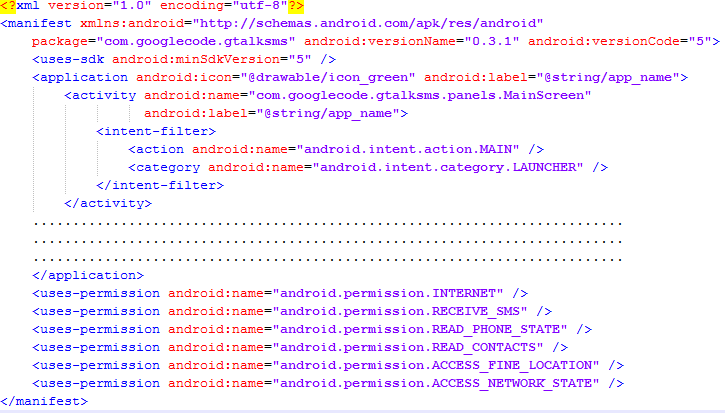
\includegraphics[height=2.4in, width=\columnwidth]{Manifest.png}
\caption{Android Manifest}
\vskip -6pt
\label{fig:Manifest}
\end{figure}

In this project, we build an efficient automated Java-based Android package analyzer called ApkExtractor which we use in conjunction with ApkTool\cite{ApkTool} for reverse engineering of APK files. Within ApkExtractor, we first invoke ApkTool to extract and decompile all the applications. Since ApkTool takes around 30s - 2 minutes to decompile an application (depending on the size), we parallelized the execution using the Executor Service (multi-threaded library) support in Java. We proceed to extract code-based features and permission-based features from the file.

\section{Feature Extraction}

\subsection{Code Based Features}

For each extracted application, we read the Manifest file to extract a list of Activity files referenced by the application. These Activity files (.smali) are decompiled versions of the original source code and contain Dalvik opcodes. For each Activity file, we only retain the opcodes and discard most operands, except the opcodes storing constant data (such as const-string) for which the resultant opcode becomes the concatenation of the opcode with the value referenced. Since each Manifest file contains multiple Activity files, we optimize the parsing by using the stream feature in Java 8, thereby representing each Manifest file as a parallel stream. For each Manifest file, we extract basic blocks (each basic block corresponds to the opcode list extracted from an Activity file) and label the basic block according to the package it came from within the application. The result of this approach is a list of labeled opcode lists (called BB file) which is then serialized for subsequent transformations. Each application corresponds to a single serialized BB file.

\subsection{JuxtApp Analysis}

\section{Permission Based Malware Detection}

\subsection{Motivation}	\label{limitJuxtApp}

Although we achieve impressive results for Juxtapp, we quickly notice that the approach suffers from some serious limitations for the case of malware detection. Firstly, We noticed that clustering reported poor results when we did not introduce the malware seed as an independent application. Secondly, JuxtApp analysis is built on the malwares it has been exposed to, and is unable to detect new types of malwares, or malicious applications infected with these malwares. Lastly, JuxtApp is a computation-intensive algorithm at least in the ApkExtractor stage, and ignores valuable information from the Manifest file. 

There is clearly a need for improved detection capabilities to overcome the aforementioned challenges and be able to successfully handle Malware evolution. We address the limitations described above by looking at the malware detection process from a more fundamental outlook. Android security mechanism depends heavily on a permission-based mechanism. While JuxtApp is busy extracting opcode lists from multiple Activity files, we utilize a tiny bit of the system resources to extract relevant permissions from the Manifest file. We explain our static-analysis approach below using permissions as features, to detect malicious applications.

\subsection{Feature Extraction} \label{featureExtract}

Permissions are described in the Manifest file via a \textit{<uses-permission>} label. For example, if the application requires active Internet connection, the corresponding permission is specified by \textit{<uses-permission
android:name="android.permission.INTERNET"/>}. Similarly, access to camera can be requested by inserting a \textit{<uses-permission android:name="android.permission.CAMERA"/>} statement within the Manifest. In total, Android exposes 150 standard user permissions\cite{Permission}. Programmers can have their own custom permissions, built over these standard set of permissions. We ignore the custom permissions since different programmers can have different permissions (curated as per their needs) and pick only those permissions from the Manifest which belong to the standard set. For each APK, we create a bit vector of size 150. We represent each APK as a vector defined by $\bar{r} = (r_{1}, r_{2}....r_{n})$, where $r_{i}$ represents the $i^{th}$ index of the feature vector obtained from the ApkExtractor. Then $r_{i}$ can be explained by the random variable:
\[
    r_i= 
\begin{cases}
    1,& \text{if extracted permission} \in \text{Android permission set} \\
    0,              & \text{otherwise}
\end{cases}
\]

Thus, we assign 1 to the index \textit{i}, if the permission corresponding to index \textit{i} is present in the Manifest of the corresponding APK. Since, applications generally tend to request a subset of the standard permission set, we compute the information gain or the Mutual Information (MI)\cite{cover2012elements} of each feature $r_{i}$ with respect to the class variable C. Using MI we select and rank the top features and use this trimmed feature set for model training. Let \textit{C} represent the application type which can be either benign or malicious. The most influential features are determined by the MI score of each APK represented by the random variable $R_{i}$ and is given by:
 \small
\begin{equation}	\label{eqMI}
MI(R_{i}, C) = \sum_{r\in { 0,1}} \sum_{C\in {mal, ben}}P(R_{i}=r;C=c)\cdot \log_2 \Big(\frac{P(R_{i}=r;C=c)}{P(R_{i}=r)\cdot P(C=c)}\Big)
\end{equation} \normalsize

We compute the information gain score for each feature vector and pick all the permissions whose feature vectors correspond to a positive information gain score. 

\begin{figure*}[htbp]
\centering
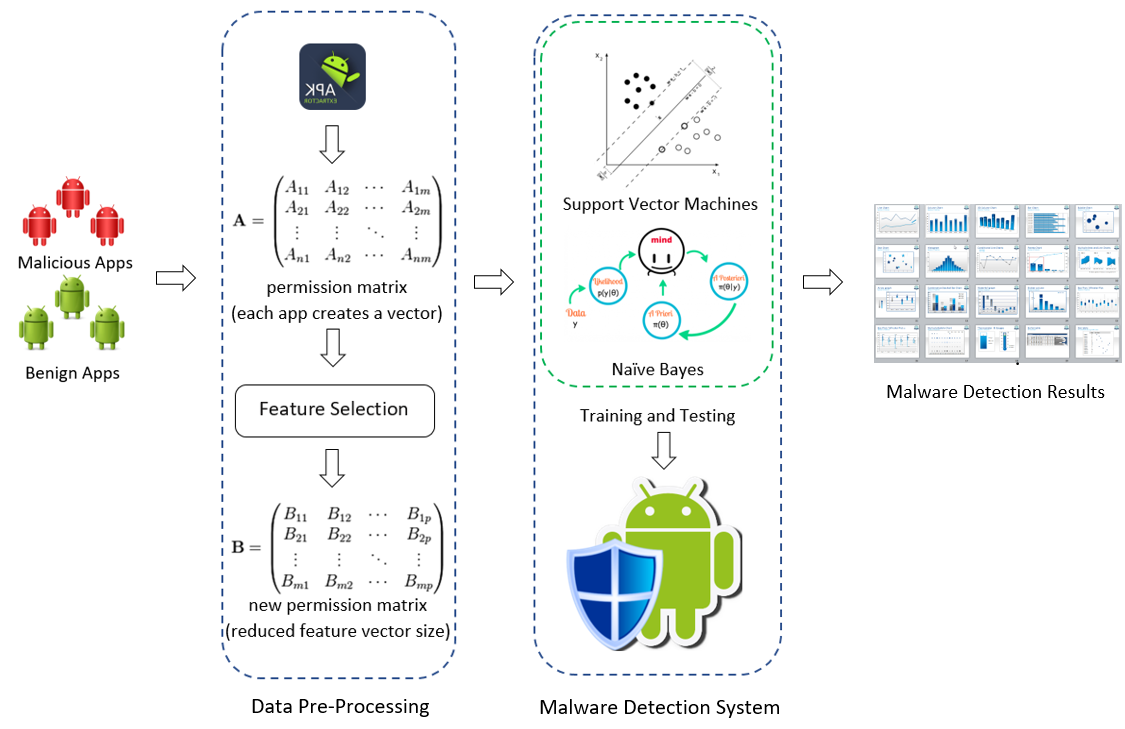
\includegraphics[width=\textwidth]{images/permFlow.png}
\caption{Flow Chart form Permission Based Malware Detection\label{permissioFlow}} 
\end{figure*}

\section{Methodology}
In order to build our model, we used 148 applications comprising of 101 benign applications and 47 malicious applications belonging to 19 different malware types. Figure \ref{permissioFlow} summaries our entire procedure. We use the ApkExtractor to extract and store permissions that belong to the standard permission set exposed by Android. We maintain a global permission list for those 150 permissions and increment the count of each extracted permission. The top 20 requested permissions extracted from the benign applications and the malware applications are shown in Table \ref{benignPerm} and \ref{maliciousPerm}. We note that the top permissions requested for both benign and malware applications are almost the same as the ones obtained by Zhou in \cite{zhou2012dissecting} who used a huge dataset of Malware samples developed in-house \cite{Genome}. We thus state that the 47 malware samples obtained from Contagio Malware Dump and 101 benign application obtained from Google Play\cite{PlayStore}, mimic and build-up on the studies previously performed on malware detection.

\small 
\begin{table}[]
\centering
\begin{tabular}{|l|l|}
\hline
\textbf{Permission}               & \textbf{Frequency} \\ \hline
INTERNET                          & 97                 \\ \hline
ACCESS\_NETWORK\_STATE            & 85                 \\ \hline
WRITE\_EXTERNAL\_STORAGE          & 50                 \\ \hline
READ\_PHONE\_STATE                & 50                 \\ \hline
ACCESS\_FINE\_LOCATION            & 49                 \\ \hline
ACCESS\_COARSE\_LOCATION          & 45                 \\ \hline
WAKE\_LOCK                        & 42                 \\ \hline
GET\_ACCOUNTS                     & 35                 \\ \hline
ACCESS\_WIFI\_STATE               & 29                 \\ \hline
VIBRATE                           & 24                 \\ \hline
ACCESS\_LOCATION\_EXTRA\_COMMANDS & 23                 \\ \hline
RECEIVE\_BOOT\_COMPLETED          & 16                 \\ \hline
CAMERA                            & 12                 \\ \hline
CALL\_PHONE                       & 10                 \\ \hline
CHANGE\_WIFI\_STATE               & 10                 \\ \hline
GET\_TASKS                        & 8                  \\ \hline
RECORD\_AUDIO                     & 7                  \\ \hline
MODIFY\_AUDIO\_SETTINGS           & 6                  \\ \hline
READ\_CONTACTS                    & 5                  \\ \hline
INSTALL\_SHORTCUT                 & 4                  \\ \hline
READ\_EXTERNAL\_STORAGE           & 4                  \\ \hline
SYSTEM\_ALERT\_WINDOW             & 4                  \\ \hline
DISABLE\_KEYGUARD                 & 4                  \\ \hline
MOUNT\_UNMOUNT\_FILESYSTEMS       & 4                  \\ \hline
RECEIVE\_SMS                      & 4                  \\ \hline
SEND\_SMS                         & 3                  \\ \hline
CHANGE\_CONFIGURATION             & 3                  \\ \hline
SET\_WALLPAPER                    & 3                  \\ \hline
WRITE\_CONTACTS                   & 3                  \\ \hline
READ\_SMS                         & 2                  \\ \hline
\end{tabular}
\caption{Top 20 Requested Permissions from 101 Benign Applications}\label{benignPerm}
\end{table}
\normalsize
Looking closely at Tables \ref{benignPerm} and \ref{maliciousPerm}, we notice that the top 20 permissions differ significantly and thus indicate the presence of discriminative capabilities. These discriminative capabilities can be used to train a classifier to distinguish between benign and malicious applications and motivate us to apply a supervised-learning approach.
\small
\begin{table}[]
\centering
\begin{tabular}{|l|l|}
\hline
\textbf{Permission}               & \textbf{Frequency} \\ \hline
INTERNET                          & 97                 \\ \hline
ACCESS\_NETWORK\_STATE            & 85                 \\ \hline
WRITE\_EXTERNAL\_STORAGE          & 50                 \\ \hline
READ\_PHONE\_STATE                & 50                 \\ \hline
ACCESS\_FINE\_LOCATION            & 49                 \\ \hline
ACCESS\_COARSE\_LOCATION          & 45                 \\ \hline
WAKE\_LOCK                        & 42                 \\ \hline
GET\_ACCOUNTS                     & 35                 \\ \hline
ACCESS\_WIFI\_STATE               & 29                 \\ \hline
VIBRATE                           & 24                 \\ \hline
ACCESS\_LOCATION\_EXTRA\_COMMANDS & 23                 \\ \hline
RECEIVE\_BOOT\_COMPLETED          & 16                 \\ \hline
CAMERA                            & 12                 \\ \hline
CALL\_PHONE                       & 10                 \\ \hline
CHANGE\_WIFI\_STATE               & 10                 \\ \hline
GET\_TASKS                        & 8                  \\ \hline
RECORD\_AUDIO                     & 7                  \\ \hline
MODIFY\_AUDIO\_SETTINGS           & 6                  \\ \hline
READ\_CONTACTS                    & 5                  \\ \hline
INSTALL\_SHORTCUT                 & 4                  \\ \hline
READ\_EXTERNAL\_STORAGE           & 4                  \\ \hline
SYSTEM\_ALERT\_WINDOW             & 4                  \\ \hline
DISABLE\_KEYGUARD                 & 4                  \\ \hline
MOUNT\_UNMOUNT\_FILESYSTEMS       & 4                  \\ \hline
RECEIVE\_SMS                      & 4                  \\ \hline
SEND\_SMS                         & 3                  \\ \hline
CHANGE\_CONFIGURATION             & 3                  \\ \hline
SET\_WALLPAPER                    & 3                  \\ \hline
WRITE\_CONTACTS                   & 3                  \\ \hline
READ\_SMS                         & 2                  \\ \hline
\end{tabular}
\caption{Top 20 Requested Permissions from 47 Malicious Applications}\label{maliciousPerm}
\end{table}
\normalsize
As described in Section \ref{featureExtract}, we perform feature selection and ranking via the principle of Information Gain as per Equation \ref{eqMI} to obtain the most influential features. The top 20 permissions based on the Mutual Information scores are shown in Table \ref{MIScore}. The resulting permission set validate the effectiveness of the permissions used. 
\small
\begin{table}[]
\centering
\begin{tabular}{|l|l|l|l|}
\hline
\textbf{Permission Name}    & \textbf{Benign} & \textbf{Malware} & \textbf{MI Score} \\ \hline
SEND\_SMS                   & 3               & 31               & 0.3521979534      \\ \hline
RECEIVE\_SMS                & 4               & 27               & 0.2637522663      \\ \hline
READ\_SMS                   & 2               & 24               & 0.2573418029      \\ \hline
RECEIVE\_BOOT\_COMPLETED    & 16              & 36               & 0.2548782512      \\ \hline
CHANGE\_NETWORK\_STATE      & 1               & 18               & 0.1934443619      \\ \hline
GET\_TASKS                  & 8               & 26               & 0.1895535975      \\ \hline
SYSTEM\_ALERT\_WINDOW       & 4               & 21               & 0.1759229822      \\ \hline
KILL\_BACKGROUND\_PROCESSES & 0               & 14               & 0.1727795965      \\ \hline
READ\_CONTACTS              & 5               & 21               & 0.1612427015      \\ \hline
WRITE\_SETTINGS             & 2               & 17               & 0.1573133865      \\ \hline
RESTART\_PACKAGES           & 1               & 15               & 0.1525972164      \\ \hline
MOUNT\_UNMOUNT\_FILESYSTEMS & 0               & 19               & 0.1497362779      \\ \hline
READ\_EXTERNAL\_STORAGE     & 4               & 19               & 0.1497362779      \\ \hline
INSTALL\_PACKAGES           & 0               & 12               & 0.1458568616      \\ \hline
READ\_PHONE\_STATE          & 50              & 43               & 0.1340806025      \\ \hline
READ\_LOGS                  & 2               & 15               & 0.1316379547      \\ \hline
INSTALL\_SHORTCUT           & 4               & 8                & 0.1249972087      \\ \hline
WRITE\_EXTERNAL\_STORAGE    & 50              & 42               & 0.1172152836      \\ \hline
CHANGE\_WIFI\_STATE         & 10              & 21               & 0.1070123592      \\ \hline
UNINSTALL\_SHORTCUT         & 0               & 8                & 0.0944492251      \\ \hline
DELETE\_PACKAGES            & 0               & 8                & 0.0944492251      \\ \hline
WRITE\_APN\_SETTINGS        & 1               & 10               & 0.0899809955      \\ \hline
GET\_PACKAGE\_SIZE          & 0               & 7                & 0.0820657149      \\ \hline
WRITE\_SECURE\_SETTINGS     & 0               & 7                & 0.0820657149      \\ \hline
CLEAR\_APP\_CACHE           & 1               & 9                & 0.0782839407      \\ \hline
RECEIVE\_MMS                & 0               & 6                & 0.0698574841      \\ \hline
SET\_ALARM                  & 0               & 6                & 0.0698574841      \\ \hline
READ\_CALL\_LOG             & 0               & 6                & 0.0698574841      \\ \hline
CALL\_PHONE                 & 10              & 17               & 0.0671520506      \\ \hline
ACCESS\_WIFI\_STATE         & 29              & 28               & 0.0611502389      \\ \hline
RECEIVE\_WAP\_PUSH          & 0               & 5                & 0.0578190439      \\ \hline
DISABLE\_KEYGUARD           & 4               & 10               & 0.0501392         \\ \hline
MODIFY\_PHONE\_STATE        & 0               & 4                & 0.0459451834      \\ \hline
PROCESS\_OUTGOING\_CALLS    & 1               & 5                & 0.0347435484      \\ \hline
READ\_CALENDAR              & 0               & 3                & 0.0342309502      \\ \hline
BATTERY\_STATS              & 0               & 3                & 0.0342309502      \\ \hline
BROADCAST\_STICKY           & 2               & 6                & 0.0325081802      \\ \hline
EXPAND\_STATUS\_BAR         & 0               & 2                & 0.0226716323      \\ \hline
BROADCAST\_PACKAGE\_REMOVED & 0               & 2                & 0.0226716323      \\ \hline
REBOOT                      & 0               & 2                & 0.0226716323      \\ \hline
\end{tabular}
\caption{Top 20 Requested Permissions based on Mutual Information Score}\label{MIScore}
\end{table}
\normalsize

The top n permissions as shown in Table \ref{MIScore} are used to construct the input feature vectors $\bar{r} = \big(r_{1}, r_{2}...r{n}\big)$ that represent each application used in the dataset. We remove all permission with a MI score of zero and obtain a trimmed feature matrix. We perform Bayesian classification on this feature set, since Bayesian methods can perform relatively fast classification with an extremely low computational overhead. By Bayes theorem, the probability of an application belonging to class C can be given by:

\begin{equation} \label{eqBayes}
P(C=c; \bar{R}=\bar{r}) = \frac{P(C=c)\prod_{i=1}^{n} P(R_{i}=r_{i}|C=c)}{\sum_{j\in {0,1}}P(C=c_{j})\prod_{i=1}^{n} {P(R_{i}=r_{i}|C=c_{i})}}
\end{equation}

where n is the number of features used and $c_{0}$ and $c_{1}$ correspond to benign and malicious classes. An application is thus classified as benign if $$P(C=benign|\bar{R}=\bar{r}) > P(C=malicious|\bar{R}=\bar{r})$$

\section{Evaluation}
For each APK, we obtain a trimmed feature vector of length 41 after removing all permissions with a MI score of 0. The feature matrix is then used to train a Bayesian classifier. We employ a 10-fold stratified cross-validation technique to provide a diverse range of samples to the classifier to test on. We first randomize the feature matrix and divide it into 10 parts; 9 out of which are used for building the model and the remaining 1 part is used for testing. We iterate over the process 10 times, such that each part is considered as a test set exactly once. Finally we average the results over the 10 iterations. We obtained impressive results without any further feature tuning. For the dataset of 147 APKs, the classifier was able to correctly classify 131 applications and reported an incorrect class for the remaining 16 instances. Table \ref{permConfMat} represents the corresponding confusion matrix Table \ref{detailAcc} represents the detailed accuracy by class

\begin{table}
  \centering%
  \begin{tabular}{|ccc|}
  \hline
 & actual benign & actual malicious \\ [0.5ex]
\hline 
pred benign & 94 & 6 \\
pred malware & 10 & 37 \\ 
\hline
  \end{tabular}
  \caption{Confusion Matrix}\label{permConfMat}
\end{table}

\small
\begin{table}[]
\centering
\begin{tabular}{|l|l|l|l|l|l|l|}
\hline
                       & \textbf{TP Rate} & \textbf{FP Rate} & \textbf{Precision} & \textbf{Recall} & \textbf{ROC Area} & \textbf{Class} \\ \hline
                       & 0.940            & 0.213            & 0.904              & 0.940           & 0.934             & benign         \\ \hline
                       & 0.787            & 0.060            & 0.860              & 0.787           & 0.934             & malicious      \\ \hline
\textbf{Weighted Avg.} & 0.891            & 0.164            & 0.890              & 0.891           & 0.934             &                \\ \hline
\end{tabular}
\caption{Detailed Accuracy by Class} \label{detailAcc}
\end{table}
\normalsize

\section{Discussion \& Conclusion}

\section{Future Work}